\documentclass[conference]{IEEEtran}
% The TALE 2026 camera-ready instructions do not ask for a first-page copyright
% block; their only copyright requirement covers self-archiving. If the
% publication chair or PDF eXpress asks for one, uncomment these lines and the
% \IEEEpubidadjcol in Section I, and fill in the proceedings ISBN.
% \IEEEoverridecommandlockouts
% \IEEEpubid{\makebox[\columnwidth]{%
%   <ISBN>/26/\$31.00~\copyright~2026 IEEE\hfill}%
%   \hspace{\columnsep}\makebox[\columnwidth]{}}
\usepackage{cite}
\usepackage{amsmath,amssymb}
\usepackage{graphicx}
\usepackage{textcomp}
\usepackage{xcolor}
\usepackage{booktabs}
\usepackage{multirow}
\usepackage{url}
\usepackage{hyperref}
\usepackage{balance}

\begin{document}
% EDAS rejects manuscripts carrying page numbers, headers or footers. The
% conference class already omits them; this makes that explicit.
\pagestyle{empty}

\title{Teaching Software Testing and Debugging Through a Serious Game: An Empirical Classroom Study with Sojourner under Sabotage}

\author{
\IEEEauthorblockN{Aazaade Faraji\IEEEauthorrefmark{1}, Enrico Nunes\IEEEauthorrefmark{1}, Francisco Reis\IEEEauthorrefmark{1}, Nuno Pombo\IEEEauthorrefmark{1}\IEEEauthorrefmark{2}, Christina Andersson\IEEEauthorrefmark{3}}
\IEEEauthorblockA{\IEEEauthorrefmark{1}Universidade da Beira Interior, Covilh\~{a}, Portugal}
\IEEEauthorblockA{\IEEEauthorrefmark{2}Instituto de Telecomunica\c{c}\~{o}es, Universidade da Beira Interior, Covilh\~{a}, Portugal}
\IEEEauthorblockA{\IEEEauthorrefmark{3}Computer Science \& Engineering, Frankfurt University of Applied Sciences, Frankfurt, Germany}
\{aazaade.faraji, enrico.nunes, francisco.reis, ngpombo\}@ubi.pt, christina.andersson@fra-uas.de
}

\maketitle
\thispagestyle{empty}

\begin{abstract}
Software testing and debugging matter in software engineering, but students often find them boring and struggle to turn theory into practice. To make the experience more concrete we ran a classroom study with \emph{Sojourner under Sabotage}, a browser-based serious game in which students write JUnit tests, build line coverage, spot mutations and debug sabotaged spaceship components across seven increasingly hard levels. We evaluated a single combined session---an introductory lecture followed by guided gameplay---with 22 master's students, collecting pre- and post-session quizzes, confidence ratings, perception surveys, open-ended feedback and in-game telemetry: 3,161 events across 14 event types. Students' confidence in analyzing test failures increased ($+0.38$; 7~improved, 0~declined), 95\% agreed the session improved their understanding of testing versus debugging, and 86\% agreed that the activity was engaging. Knowledge gains were positive but not statistically significant (exact Wilcoxon $p = 0.117$), which a high pre-test baseline largely explains. Telemetry showed that students who progressed further also tended to improve more on the quiz (Spearman $\rho = 0.53$, permutation $p = 0.015$, 95\%~CI $[0.12, 0.78]$). Because the lecture and the game were delivered together and no control group was used, these findings are exploratory: they describe associations rather than establishing that the game itself caused the observed gains.

\end{abstract}

% First five are IEEE Taxonomy (Jan 2026) terms, verbatim, so IEEE indexes them;
% "Learning analytics" is not in the taxonomy but is what this community searches.
\begin{IEEEkeywords}
Software testing, Debugging, Serious games, Computer science education, Educational technology, Learning analytics
\end{IEEEkeywords}

% ===========================================================================
\section{Introduction}
\label{sec:intro}
% ===========================================================================
In software engineering, testing and debugging skills are crucial, but students often find them boring and tedious compared to coding~\cite{straubinger2023survey, garousi2020testing}. Traditional lecture-based teaching has a hard time keeping their attention and leaves a large gap between theoretical understanding and real-world application~\cite{mccauley2008debugging}. Game-based teaching can recast testing tasks as narrative-driven gameplay with immediate, tangible feedback~\cite{connolly2012systematic, blanco2023gamification}.
\emph{Sojourner under Sabotage}~\cite{straubinger2025sojourner} is a browser-based serious game in which players repair sabotaged spaceship systems by writing JUnit tests and debugging mutated code across seven levels; an initial evaluation with 79~students reported over 80\% enjoyment and measurable improvements in test coverage and debugging skills.
This paper extends that work with an independent evaluation in a different institutional context: a self-hosted instance for 22 master's students at a Portuguese university, combining pre/post knowledge assessments, self-confidence measures, perception questionnaires, open-ended feedback and fine-grained behavioral telemetry (3,161 events across 14 types). That lets us ask not only \emph{whether} scores and attitudes shift over the session, but also \emph{how} students engage with the tasks during gameplay.

% \IEEEpubidadjcol  % re-enable only together with the \IEEEpubid block above
Three questions guide the study. \textbf{RQ1}: to what extent do students' conceptual understanding and self-assessed confidence change over the session? \textbf{RQ2}: how do they perceive the game in terms of engagement, perceived learning, usability and cognitive load? \textbf{RQ3}: what behavioral patterns emerge from the telemetry, and how do they relate to learning outcomes? RQ1 and RQ2 are the primary evaluation; RQ3 adds a second view of the same session.
The contribution is an independent evaluation outside the group that built the game and---absent from earlier evaluations---a telemetry-based account of how students actually behaved during play.

% ===========================================================================
\section{Background and Related Work}
\label{sec:background}
% ===========================================================================

Software testing is often taught inside general programming courses and is widely perceived as tedious~\cite{garousi2020testing, straubinger2023survey}; debugging receives even less instructional focus, and novices struggle with misconceptions about program behavior~\cite{mccauley2008debugging}. This has motivated strategies grounded in experiential and problem-based learning~\cite{kolb1984experiential, hmelo2004problem}.

Gamification has shown promise in testing education~\cite{blanco2023gamification}, though poor design can cause frustration~\cite{toda2017dark}, and serious games offer immersive, goal-driven experiences~\cite{connolly2012systematic}.
Several target testing: the Testing Game~\cite{valle2017testing} teaches strategies but lacks hands-on test writing; Code Defenders~\cite{fraser2019code} engages students with JUnit and mutations but has usability concerns; Code Critters~\cite{straubinger2023code} targets younger learners.

By exercising fault localization, mutation detection and iterative refinement, \emph{Sojourner under Sabotage}~\cite{straubinger2025sojourner} pushes students past the verification-oriented habit of confirming expected outputs. Unlike the previous evaluations, which were conducted by the game's developers, ours is an \emph{independent replication} in a different institutional and cultural context, with telemetry-based behavioral analysis added.

% ===========================================================================
\section{Methodology}
\label{sec:methodology}
% ===========================================================================

\subsection{Participants and Context}

Participants were 22 master's students enrolled in a software engineering course at a Portuguese university.
Most (21/22) were from Computer Science or Software Engineering programs.
Self-reported programming experience was predominantly intermediate (14/22), with basic testing (17/22) and debugging (15/22) experience.
Only 8/22 had prior experience with testing tools.

\textbf{Ethics and data governance.}
Participation was voluntary and based on informed consent obtained at the start of the questionnaire; students could decline without any effect on their course standing. The activity was run as part of regular coursework and no sensitive personal data were collected.
Students chose a self-generated participant code, which was the only key linking questionnaire responses to game accounts; no names, student numbers, or IP addresses were recorded.
The linked data were stored on the research group's internal server, accessible only to the authors, and the released replication package contains pseudonymized data only.

\subsection{The Game: Sojourner under Sabotage}

Each of the seven levels runs as a cycle: a robot companion introduces a component; the player writes JUnit tests until they reach $\geq$50\% line coverage, at which point the tests are activated to monitor for sabotage; the system injects a mutation; and if the tests catch it, the player locates and fixes the fault. If the mutation goes undetected the component is ``destroyed'' and a hidden test is supplied as scaffolding.
Each student's game username matched their questionnaire participant code, which is what links telemetry, pre-test and post-test data per student.

\subsection{Deployment and Monitoring Infrastructure}

We deployed the instance on the university's internal server, reachable over the institutional network, and generated anonymous accounts in bulk through the game's administrative interface. For post-session analysis we built a small web dashboard over the game's JSON telemetry export, so instructors can inspect a student's testing and debugging actions without reading raw JSON.

\subsection{Session Structure}
The session lasted approximately 2 hours, of which 50 minutes were an introductory lecture on software testing concepts, and the next approximately 60 minutes were devoted to guided gameplay, with 10 minutes allocated to completing pre- and post-activity questionnaires.
The post-test therefore followed \emph{both} components: the design cannot separate the lecture's contribution from the game's, and we interpret all results accordingly.

\subsection{Data Collection}

The pre-activity questionnaire collected background information, 11~multiple-choice question (MCQ) items spanning testing vs.\ debugging, the unit/integration/black-box/white-box/mutation/functional distinctions and test case analysis, and four self-confidence Likert items (5-point scale). The post-activity questionnaire repeated those and added perceived learning (4~items), engagement (3), usability (3), cognitive load (3) and four open-ended questions; the full instrument is in the replication package.
In parallel the backend logged 14~event types per player, covering room and phase transitions, edits to the test class and the class-under-test, test results with per-method pass/fail and coverage, compilation errors, mutation outcomes, component fixes and destructions, and hidden test triggers.

\subsection{Data Analysis}

All analyses were computed with SciPy~1.13; the script is in the replication package.
MCQ scores were compared with a two-sided Wilcoxon signed-rank test. The seven zero differences were discarded, leaving $n = 14$ non-zero pairs, and tied absolute differences were handled by mid-ranks. We report an exact $p$-value obtained by enumerating all $2^{14}$ sign assignments of the observed ranks; the tie-corrected normal approximation is given alongside it. The effect size is $r = |Z|/\sqrt{N}$ with $N = 21$ pairs.
Normalized learning gain was computed as $g = (post - pre)/(11 - pre)$.
Spearman correlations were estimated as Pearson correlations on mid-ranks (valid under ties) and tested with a permutation test over $10^5$ pairings; 95\% confidence intervals use the Fisher $z$ transform.
Internal consistency was assessed using Cronbach's~$\alpha$ for every multi-item scale.
Questionnaire constructs are reported as means; ``\% agree'' denotes responses of 4 or 5 on the 5-point scale, and a construct's \% agree is the mean of its items' individual percentages.

% ===========================================================================
\section{Results}
\label{sec:results}
% ===========================================================================

\subsection{RQ1: Knowledge and Confidence}

\subsubsection{MCQ Knowledge Assessment}

Across the 21 matched pairs (22 pre, 21 post), the mean score rose from 8.29 (median 8, IQR 8--9) to 9.14 out of 11 (median 10, IQR 8--10; $\Delta = +0.86$, normalized gain 0.246), with 10 students improving, 7 unchanged and 4 declining.
The Wilcoxon test was not significant ($T = 27$, $n = 14$, $Z = 1.627$, exact $p = 0.117$; $r = 0.355$, medium).
The improvement is therefore a positive but statistically inconclusive trend.
Descriptively, the three students scoring below 8 at pre-test gained most (5.67~$\rightarrow$~9.00, normalized gain 0.50), the fifteen mid-baseline students gained moderately (8.40~$\rightarrow$~8.93, 0.244), and the three scoring $\geq 10$ did not change.
These cut-offs were chosen after inspecting the distribution and the extreme groups contain only three students each, so the pattern is descriptive only: regression to the mean and the narrower headroom available to high scorers are equally plausible explanations, and we draw no inference about differential benefit.

Per-item accuracy improved most on concepts directly practiced in the session: the testing vs.\ debugging distinction (+26\%), revealing test case identification (+22\%), and mutation testing (+12\%). Items already near ceiling at pre-test (Q3, Q4, Q10, Q11; $\geq 95\%$ correct) did not change; per-item pre-test accuracy ranged from 41\% to 100\%.

\subsubsection{Self-Confidence}

All four self-confidence items improved on the 5-point scale: understanding concepts 3.43~$\rightarrow$~3.57, writing a test case 3.48~$\rightarrow$~3.71, identifying and debugging errors 3.48~$\rightarrow$~3.67, and analyzing test failures 3.24~$\rightarrow$~3.62. The last is the largest gain ($+0.38$) and the only item no student rated lower afterwards (7~improved, 14~unchanged, 0~declined).
Internal consistency was good (Cronbach $\alpha_{pre} = 0.814$, $\alpha_{post} = 0.848$).

\subsection{RQ2: Student Perception}

Students rated the session highly on all three reliable constructs: perceived learning 4.06 (86\% agree, $\alpha = 0.87$), engagement 4.05 (76\%, $\alpha = 0.75$) and usability 4.24 (75\%, $\alpha = 0.98$).
At the level of individual items, 95\% agreed it helped them understand testing vs.\ debugging, 86\% agreed the activity was engaging, and 71\% preferred it over traditional lectures.
The three cognitive-load items did not form a reliable scale ($\alpha = -0.57$), so we report them individually rather than as a composite: mental effort 3.19, parts of the activity confusing 2.86, and difficulty level appropriate 3.86 (71\% agreement).

One author grouped the open-ended responses by recurring topic. This was not a formal thematic analysis with independent coders, so we report the groupings as descriptive impressions, with counts out of 21 respondents.
Asked what helped them learn most, 8 named the game or its interactivity (\emph{``The code changing in real time demanding debugging''}) and 3 credited the preceding lecture, slides or instructor.
Asked what was hardest, 6 pointed to writing or designing the tests, 5 to understanding the code and locating faults, and 4 to orienting themselves when the game began (\emph{``know where to start''}). Only 3 raised the programming language itself (\emph{``Sintaxe do Java''}; one asked for Python).

\subsection{RQ3: Behavioral Engagement (Telemetry)}

The game recorded 3,161~events across 14 event types from the 22~students who played (Table~\ref{tab:telemetry}); the 21 who also completed both questionnaires form the matched set used below, and a further unmatched account's 15~events are excluded throughout.
For those 21, a median of 40~minutes separated their first and last logged event, or 32~minutes with any gap longer than five minutes capped at five to discount idle time.

\begin{table}[htbp]
\caption{Telemetry event counts (22 students, 3,161 logged records). Component fixed, mutation detected and destroyed are logged twice per occurrence: 53, 34 and 28 distinct.}
\label{tab:telemetry}
\centering
\small
\begin{tabular}{lr@{\hskip 1.2em}lr}
\toprule
Event & $n$ & Event & $n$ \\
\midrule
Room unlocked      & 1,297 & CUT modified        & 89 \\
Game progression   & 420   & Mutation detected   & 68 \\
Conversation       & 319   & Tests activated     & 61 \\
Test modified      & 276   & Debug started       & 58 \\
Test executed      & 219   & Component destroyed & 56 \\
Test exec.\ failed & 113   & Game started        & 43 \\
Component fixed    & 106   & Hidden test added   & 36 \\
\bottomrule
\end{tabular}
\end{table}

Progression fell off steadily: all 22 students started Room~1 (CryoSleep), 16 (73\%) reached Room~2, then 11, 10, 8 and 6 students reached Rooms~3--6 respectively, and 2 (9\%) reached Room~7; no student completed it.

Fifty-six \emph{ComponentDestroyedEvent}s---28 distinct cases, since the game logs each destruction twice---indicate where students' tests failed to detect sabotage, triggering hidden tests as scaffolding (36~events).
The counts show the scaffolding was triggered in practice, say nothing about whether it improved learning, and are concentrated in a subset of students.
An exploratory correlation analysis ($N = 21$ students with matched telemetry and questionnaire data) found a positive association between game progression and MCQ gains (Spearman $\rho = 0.53$, permutation $p = 0.015$, 95\%~CI $[0.12, 0.78]$; Fig.~\ref{fig:correlation}).
Progression was also strongly correlated with test executions ($\rho = 0.91$, $p < 0.001$, CI $[0.79, 0.96]$), although advancement in this game structurally \emph{requires} executing tests, so this association is partly a property of the design rather than an independent finding.

\begin{figure}[htbp]
\centering
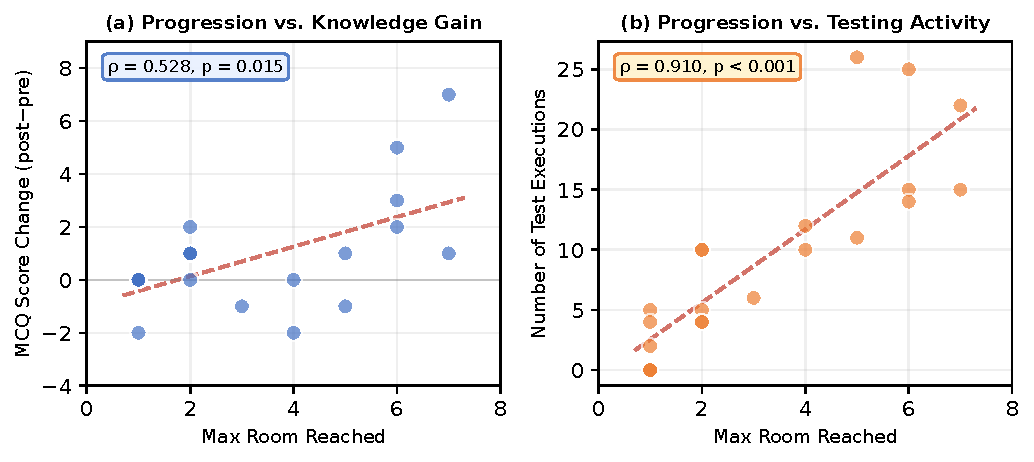
\includegraphics[width=\columnwidth]{figures/fig_correlation.pdf}
\caption{(a) Game progression vs.\ MCQ gains ($\rho = 0.53$, $p = 0.015$). (b) Progression vs.\ test executions ($\rho = 0.91$, $p < 0.001$).}
\label{fig:correlation}
\end{figure}

% ===========================================================================
\section{Discussion}
\label{sec:discussion}
% ===========================================================================

\subsection{Interpreting the Results}

Our single-item engagement (86\%) and perceived-learning (95\%) figures are consistent with the original evaluation's report of over 80\% enjoyment~\cite{straubinger2025sojourner}, which suggests the game is received similarly outside the group that built it.
The knowledge result is weaker and needs care. The non-significant improvement (exact $p = 0.117$) is not evidence of ineffectiveness, but neither is it evidence of learning: the pre-test mean of 8.3/11 left little room to move, and four of the eleven items were already answered correctly by at least 95\% of students beforehand.
Students who progressed further did tend to improve more ($\rho = 0.53$, CI $[0.12, 0.78]$), but the interval is wide and prior knowledge, Java proficiency, motivation, working speed and time on task would all plausibly raise both progression and score change. With this sample we could not model those jointly, so progression is not independent evidence that the session produced learning.
The open-ended answers point the same way: students valued the immediate feedback and several described watching a component break and repairing it as what made testing and debugging feel different, while three credited the lecture or the instructor rather than the game---consistent with our inability to separate the two.

Two patterns in the telemetry carry a lesson for anyone running this game in class. The first is pacing. Only 2 of 22 students reached the seventh room and fewer than half got past the fourth, so an hour of play exercises the early components thoroughly and the later ones barely at all. The game's seven levels are not a syllabus that fits a single session, and treating the last of them as assessable would penalise students for the clock rather than for their testing.
The second is how much of the difficulty sat in writing tests rather than in reading code. Of 332 test-run attempts, 113 never compiled---mostly Java syntax errors in the first room---while 65 of the 219 that did compile ended in a failing test. Syntax blocks the opening level, but six students named test design as the hardest part against three who named the language: a class needs a short Java refresher up front and, beyond it, worked examples of what a useful test looks like.

\subsection{Practical Implications}

For an instructor this translates into four things: allow at least 70~minutes and plan for partial completion rather than assessing the later levels; budget guidance for the first level, where orientation and Java syntax were both obstacles; watch the failure rate live in the telemetry and step in when a student stalls on it; and say beforehand what a destroyed component means, so it is not read as personal failure.

% ===========================================================================
\section{Threats to Validity}
\label{sec:threats}
% ===========================================================================

\textbf{Internal.} A single-group pre/post design without a control group rules out causal interpretation, and with the lecture and the gameplay in one session no result can be attributed to the game alone. Reusing identical MCQ items may add a testing effect, and the instrument's ceiling limits the observable range.

\textbf{Construct.} The 11-item MCQ was written by the authors and neither externally validated nor piloted; it is in the replication package for others to assess. We report no internal-consistency coefficient for it: its items deliberately span distinct concepts rather than one latent trait, so a coefficient like KR-20 would penalise that breadth rather than measure adequacy. The cognitive-load items mix valence---one is positively worded---and were analysed in their original direction; they did not form a reliable scale, so we report them individually; usability's $\alpha = 0.98$ suggests its items are near-redundant. Perceived learning is self-report, not demonstrated learning.

\textbf{External and reliability.} A single intact class at one institution fixed the sample rather than letting us size it, so a sampling formula such as Cochran's does not apply; with $N = 21$ matched pairs the study is underpowered for anything but a large effect, and every inferential result should be read as exploratory.

% ===========================================================================
\section{Conclusion}
\label{sec:conclusion}
% ===========================================================================

We reported an exploratory evaluation of a combined lecture-and-game session built around \emph{Sojourner under Sabotage} with 22 master's students. Students rated it highly (86\% engaging, 95\% that it clarified testing vs.\ debugging) and their confidence in analyzing test failures rose, while knowledge gains were positive but not significant (exact $p = 0.117$) against a high baseline. Telemetry from 3,161 events showed that students who progressed further also tended to improve more ($\rho = 0.53$, CI $[0.12, 0.78]$).
With the two components delivered together, no control group and a small cohort, these results describe a feasible and well-received deployment and an association worth testing properly---not evidence that the game caused the gains. Future work should separate the components with a comparison condition, calibrate the instrument to the population, and follow retention beyond one session.

\section*{Data Availability}
The replication package---the full MCQ and questionnaire instruments, pseudonymized participant-level data, the telemetry export, and the analysis script that produces every number reported here---is available at \url{https://github.com/aazaadef/sojourner-tale2026}.

\section*{Acknowledgment}
This work was supported by FCT -- Funda\c{c}\~{a}o para a Ci\^{e}ncia e Tecnologia, I.P., project reference UIDB/50008/2020 (DOI: 10.54499/UIDB/50008/2020) and doctoral grant PRT/BD/155023/2023.
Generative AI tools were used solely for English language polishing. All technical content, interpretations and conclusions were created and verified by the authors, who take full responsibility for the manuscript.

\balance
\bibliographystyle{IEEEtran}
\begin{thebibliography}{99}
\bibitem{straubinger2023survey} P.~Straubinger and G.~Fraser, ``A Survey on What Developers Think About Testing,'' in \emph{Proc.\ ISSRE '23}, IEEE, 2023, pp.~80--90.
\bibitem{garousi2020testing} V.~Garousi, A.~Rainer, P.~Lauv\aa{}s~Jr., and A.~Arcuri, ``Software-testing education: A systematic literature mapping,'' \emph{J.\ Syst.\ Softw.}, vol.~165, 2020.
\bibitem{mccauley2008debugging} R.~McCauley et~al., ``Debugging: a review of the literature from an educational perspective,'' \emph{Comput.\ Sci.\ Educ.}, vol.~18, no.~2, pp.~67--92, 2008.
\bibitem{connolly2012systematic} T.~M.~Connolly et~al., ``A systematic literature review of empirical evidence on computer games and serious games,'' \emph{Comput.\ Educ.}, vol.~59, no.~2, pp.~661--686, 2012.
\bibitem{blanco2023gamification} R.~Blanco et~al., ``Can gamification help in software testing education?'' \emph{J.\ Syst.\ Softw.}, vol.~200, 2023.
\bibitem{straubinger2025sojourner} P.~Straubinger, T.~Greller, and G.~Fraser, ``Sojourner under Sabotage: A Serious Testing and Debugging Game,'' in \emph{Proc.\ FSE Companion '25}, ACM, 2025.
\bibitem{kolb1984experiential} D.~A.~Kolb, \emph{Experiential Learning: Experience as the Source of Learning and Development}. Prentice-Hall, 1984.
\bibitem{hmelo2004problem} C.~E.~Hmelo-Silver, ``Problem-Based Learning: What and How Do Students Learn?'' \emph{Educ.\ Psychol.\ Rev.}, vol.~16, no.~3, pp.~235--266, 2004.
\bibitem{toda2017dark} A.~M.~Toda et~al., ``The Dark Side of Gamification,'' in \emph{HEFA '17}, Springer, 2017, pp.~143--156.
\bibitem{valle2017testing} P.~H.~D.~Valle et~al., ``The Testing Game,'' in \emph{Proc.\ SBES '17}, 2017.
\bibitem{fraser2019code} G.~Fraser et~al., ``Gamifying a Software Testing Course with Code Defenders,'' in \emph{Proc.\ SIGCSE '19}, ACM, 2019, pp.~571--577.
\bibitem{straubinger2023code} P.~Straubinger, L.~Caspari, and G.~Fraser, ``Code Critters: A Block-Based Testing Game,'' in \emph{Proc.\ ICST '23 Workshops}, IEEE, 2023, pp.~426--429.
\end{thebibliography}

\end{document}
